% ============================================================================
%  Time-step restrictions for explicit integration of damped moving-load
%  beam problems, and two remedies.
%  Technical note -- B.Sc. Computational Engineering Science (CES), RWTH Aachen
%
%  COMPILE: tectonic note.tex   (or pdflatex note.tex, run twice).
%  All numbers and figures are produced by  python note/make_note_figures.py
% ============================================================================
\documentclass[11pt,a4paper]{article}

\usepackage[T1]{fontenc}
\usepackage[utf8]{inputenc}
\usepackage{lmodern}
\usepackage[margin=2.3cm]{geometry}
\usepackage{amsmath,amssymb}
\usepackage{graphicx}
\usepackage{booktabs}
\usepackage{siunitx}
\usepackage{caption}
\usepackage{subcaption}
\usepackage[hidelinks]{hyperref}
\usepackage{xcolor}
\usepackage{textcomp}
\usepackage{enumitem}

\sisetup{detect-all}
\graphicspath{{figures/}}
\captionsetup{font=small,labelfont=bf}
\setlist{nosep,leftmargin=1.4em}

% --- RWTH house colours + banner -------------------------------------------
\definecolor{rwthblue}{HTML}{00549F}
\definecolor{rwthblue25}{HTML}{C7DDF2}
\definecolor{rule}{HTML}{8EBAE5}
\newcommand{\rwthbanner}{%
  \noindent\colorbox{rwthblue}{%
    \parbox{\dimexpr\textwidth-2\fboxsep\relax}{%
      \vspace{2.5pt}%
      {\color{white}\textbf{RWTH AACHEN UNIVERSITY}}\hfill
      {\color{white}\footnotesize Computational Engineering Science}%
      \vspace{2.5pt}}}%
  \vspace{1pt}\par\noindent{\color{rule}\rule{\textwidth}{1.3pt}}%
}

\newcommand{\wmax}{\omega_{\max}}

\begin{document}

% ---- title block -----------------------------------------------------------
\rwthbanner
\vspace{0.8em}

{\raggedright
  {\LARGE\bfseries Time-step restrictions for explicit integration of damped
   moving-load beam problems, and two remedies}\\[0.8em]
  {\normalsize Muhammet Emir Fil}\\[0.15em]
  {\small B.Sc.\ Computational Engineering Science, RWTH Aachen
   \quad\textbullet\quad Technical note, \today}\par
}
\vspace{0.6em}
\noindent{\color{rule}\rule{\textwidth}{0.6pt}}
\vspace{1.0em}

% ---- AIM -------------------------------------------------------------------
\noindent\colorbox{rwthblue25}{%
  \parbox{\dimexpr\textwidth-2\fboxsep\relax}{%
  \vspace{3pt}\textbf{Summary.} When a damped Euler--Bernoulli beam under a
  moving load is marched with an explicit Runge--Kutta scheme, the stable time
  step is set neither by the load speed nor by the few physically relevant low
  modes: it is throttled by the \emph{stiffness-proportional} part of Rayleigh
  damping acting on the highest, mesh-dependent finite-element modes. For a
  realistic \SI{40}{m} highway overpass at \SI{2}{\percent} damping this shrinks
  the explicit step by a factor of \(\approx 13\), which raises the cost of speed
  sweeps and Monte-Carlo studies. Two standard remedies remove the
  restriction at fixed accuracy: an implicit Newmark-\(\beta\) integrator
  (\(\approx 10^3\times\) larger step, identical dynamic amplification) and
  modal truncation (three modes reproduce the response to \(0.16\,\%\) while
  enlarging the stable explicit step by \(\approx 226\times\)). Every result is
  checked against the Fr\'yba closed-form solution and reproduced by a single
  numpy-only script.\vspace{3pt}}}

\vspace{1.0em}

% ===========================================================================
\section{Motivation}
% ===========================================================================
Vehicle--bridge interaction (VBI) studies routinely require not one simulation
but \emph{many}: the dynamic amplification factor (DAF) as a function of crossing
speed, parameter sweeps over vehicle mass and damping, and Monte-Carlo ensembles
for Bridge Weigh-in-Motion and drive-by monitoring. The per-run cost is therefore
the practical bottleneck. Marching the semi-discrete equation of motion with an
explicit integrator is attractive, being trivial to implement and needing no
linear solve, but explicit schemes are only \emph{conditionally} stable, and
on a damped finite-element (FE) beam the condition is much more restrictive
than for the undamped problem. This note isolates and quantifies that
restriction on a concrete bridge and checks the two standard remedies against
an analytical reference.

% ===========================================================================
\section{Model and integrators}
% ===========================================================================
A simply-supported uniform beam of span \(L\), bending stiffness \(EI\) and mass
per length \(\bar m\) is discretised with two-node Euler--Bernoulli elements
(transverse deflection and rotation per node, consistent mass), giving
\begin{equation}
  \mathbf M\,\ddot{\mathbf u}(t) + \mathbf C\,\dot{\mathbf u}(t)
  + \mathbf K\,\mathbf u(t) = \mathbf F(t),
  \label{eq:eom}
\end{equation}
where \(\mathbf F(t)\) is the consistent nodal load of a constant point force
\(P\) moving at speed \(v\), placed each step through the element shape functions.
Damping is classical Rayleigh damping
\(\mathbf C = \alpha\mathbf M + \beta\mathbf K\), with \(\alpha,\beta\) fixed by a
target ratio \(\zeta\) at the first two natural frequencies. Two beams are used
throughout: a \SI{20}{m} span for which the Fr\'yba closed form is the exact
ground truth, and a realistic \SI{40}{m} overpass
(\(EI=\SI{8.4e10}{N.m^2}\), \(\bar m=\SI{12000}{kg/m}\),
first frequency \(f_1=\SI{2.60}{Hz}\)) for the stability and cost story.

Three integrators act on \eqref{eq:eom}: \emph{(i)} classic explicit RK4 on the
first-order state-space form; \emph{(ii)} implicit Newmark-\(\beta\)
(average acceleration, \(\gamma=\tfrac12,\ \beta=\tfrac14\)); and \emph{(iii)}
RK4 on the modally reduced system (Section~\ref{sec:remedies}). All three share
the same assembly and the same Fr\'yba reference.

% ===========================================================================
\section{The damping-dominated step restriction}
% ===========================================================================
RK4 is stable only where its growth factor satisfies \(|R(\lambda\,\Delta t)|\le1\)
for every eigenvalue \(\lambda\) of the semi-discrete system. The relevant part
of the stability region has two edges. For the \emph{undamped} structure the
eigenvalues are purely imaginary, \(\lambda=\pm i\omega\), and RK4 is stable up to
\(\omega\,\Delta t \lesssim 2\sqrt2\approx2.83\); the integrator therefore caps
the step at \(\Delta t \le 1.8/\wmax\) (a safety factor below \(2.83\)), where
\(\wmax\) is the highest FE frequency. Because the consistent-mass beam has very
stiff, mesh-dependent high modes, \(\wmax\) is already large
(\(\approx\SI{3.3e4}{rad/s}\) for the \SI{40}{m} mesh).

Stiffness-proportional damping tightens the limit further.
The modal form of \eqref{eq:eom} with \(\mathbf C=\beta\mathbf K\) gives, for a
mode of frequency \(\omega\),
\begin{equation}
  \ddot q + \beta\omega^{2}\dot q + \omega^{2} q = f(t),
  \qquad
  \lambda = \tfrac12\!\left(-\beta\omega^{2}\pm\sqrt{\beta^{2}\omega^{4}-4\omega^{2}}\right).
\end{equation}
For the high modes \(\omega\gg 2/\beta\) the discriminant is positive: the mode is
\emph{over-damped} and one root is a large negative real number,
\(\lambda \approx -\beta\omega^{2}\). RK4's stability region reaches only to
\(\approx-2.78\) along the negative real axis, so these modes impose
\begin{equation}
  \Delta t \;\le\; \frac{2.2}{\beta\,\wmax^{2}}
  \qquad(\text{real-axis limit, safety factor below }2.78).
  \label{eq:damped-cap}
\end{equation}
The ratio of the two caps is
\begin{equation}
  \frac{\Delta t_{\text{undamped}}}{\Delta t_{\text{damped}}}
  = \frac{1.8/\wmax}{2.2/(\beta\wmax^{2})}
  = 0.82\,\beta\,\wmax .
  \label{eq:ratio}
\end{equation}
For the \SI{40}{m} bridge at \(\zeta=\SI{2}{\percent}\)
(\(\beta=\SI{4.90e-4}{s}\), \(\wmax=\SI{3.32e4}{rad/s}\)) this is
\(\mathbf{13.3}\): adding realistic damping cuts the explicit step from
\(\Delta t=\SI{5.42e-5}{s}\) to \(\SI{4.07e-6}{s}\)
(Figure~\ref{fig:restriction}). The step is now governed by
\(\beta\wmax^{2}\), a product of the damping model and the \emph{mesh}, not of
any physical time scale of the problem.

\begin{figure}[t]
  \centering
  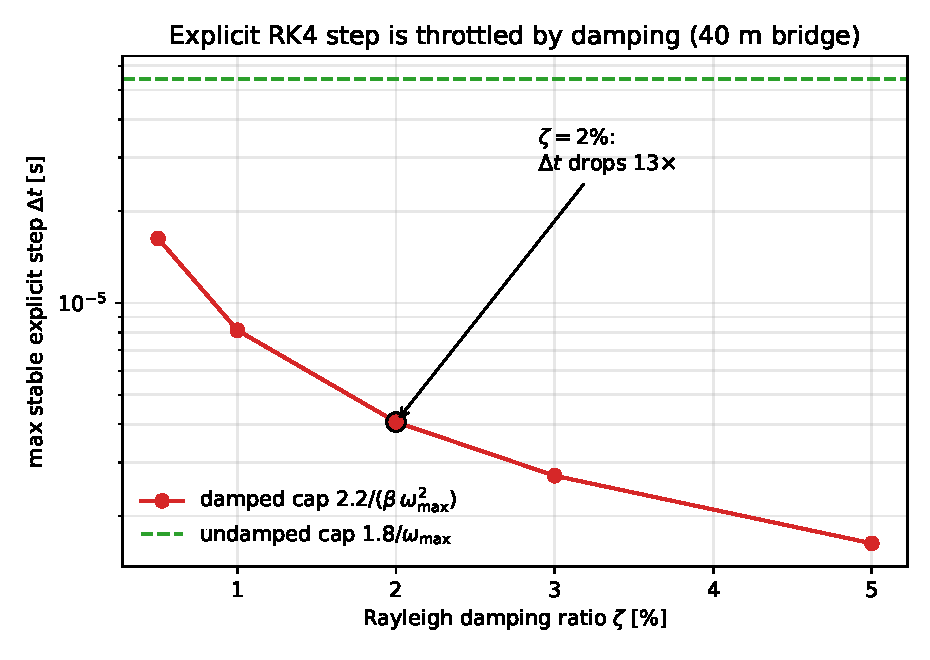
\includegraphics[width=0.62\textwidth]{restriction.pdf}
  \caption{Maximum stable explicit (RK4) time step for the \SI{40}{m} bridge as a
  function of the Rayleigh damping ratio. The undamped cap \(1.8/\wmax\) (green)
  applies only at \(\zeta=0\); any stiffness-proportional damping moves the limit
  to the \(2.2/(\beta\wmax^{2})\) branch, which scales as \(1/\zeta\) and is
  already \(13\times\) smaller at \(\zeta=\SI{2}{\percent}\).}
  \label{fig:restriction}
\end{figure}

% ===========================================================================
\section{Two remedies}\label{sec:remedies}
% ===========================================================================
\paragraph{(a) Implicit integration (Newmark-\(\boldsymbol\beta\)).}
The average-acceleration Newmark scheme is unconditionally stable for
\(\gamma\ge\tfrac12,\ \beta\ge\tfrac14\): the step is then chosen by
\emph{accuracy}, not stability. With a fixed step its effective stiffness is
factorised once. On the damped \SI{40}{m} bridge Newmark runs at
\(\Delta t=\SI{4e-3}{s}\), \(\mathbf{983\times}\) larger than the explicit cap,
and gives the same answer: DAF \(1.0800\) versus \(1.0799\), a
relative difference of \(\num{6.8e-5}\) (Table~\ref{tab:summary},
Figure~\ref{fig:remedies}b). Accuracy against Fr\'yba converges at the expected
second order in \(\Delta t\) (Figure~\ref{fig:validation}b).

\paragraph{(b) Modal truncation.}
Projecting \eqref{eq:eom} onto the first \(r\) mass-normalised eigenmodes,
\(\mathbf u=\boldsymbol\Phi\mathbf q\) with
\(\boldsymbol\Phi^{\!\top}\mathbf M\boldsymbol\Phi=\mathbf I\) and
\(\boldsymbol\Phi^{\!\top}\mathbf K\boldsymbol\Phi=\operatorname{diag}(\omega_i^2)\),
decouples the dynamics into \(r\) scalar oscillators. The reduced system's highest
frequency is the retained \(\omega_r\), not \(\wmax\), so by
\eqref{eq:damped-cap} the stable explicit step grows by \((\wmax/\omega_r)\)
undamped and by \((\wmax/\omega_r)^2\) under stiffness-proportional damping. For
the \SI{20}{m} beam, \(r=3\) modes already reproduce the peak deflection to
\(0.16\,\%\) (Figure~\ref{fig:remedies}a) while reducing \(40\) free DOFs to
\(3\) (\(13\times\)) and enlarging the undamped stable step \(226\times\)
(\(\wmax=\SI{7.27e4}{rad/s}\to\omega_3=\SI{322}{rad/s}\)). Modal truncation is the
cheaper route when a handful of modes carry the response, as they do for a
single-span bridge under traffic loads.

\begin{table}[t]
  \centering
  \caption{Damped \SI{40}{m} bridge (\(\zeta=\SI{2}{\percent}\), \(P=\SI{300}{kN}\),
  \(v=\SI{25}{m/s}\)): explicit RK4 versus implicit Newmark over one crossing.
  Same dynamic amplification, three orders of magnitude fewer steps.}
  \label{tab:summary}
  \begin{tabular}{lccc}
    \toprule
    integrator & \(\Delta t\) [s] & steps / crossing & DAF \\
    \midrule
    explicit RK4      & \num{4.07e-6} & \num{393039} & \num{1.0799} \\
    implicit Newmark  & \num{4.0e-3}  & \num{400}    & \num{1.0800} \\
    \midrule
    ratio             & \(983\times\) & \(983\times\) & \(\num{6.8e-5}\) rel. \\
    \bottomrule
  \end{tabular}
\end{table}

% ===========================================================================
\section{Verification}
% ===========================================================================
Every integrator is checked against the Fr\'yba closed-form moving-force solution
on the \SI{20}{m} span (Figure~\ref{fig:validation}a). At \(v=\SI{30}{m/s}\) the
peak mid-span deflection matches Fr\'yba to a relative error of \num{5.6e-6}
(explicit RK4), \num{2.4e-4} (Newmark, \(\Delta t=\SI{1e-3}{s}\)) and
\num{1.6e-3} (modal, \(r=3\)); the full-model DAF is \(1.1417\). These agreements
establish that the large-step remedies of Section~\ref{sec:remedies} change the
\emph{cost}, not the answer.

\begin{figure}[t]
  \centering
  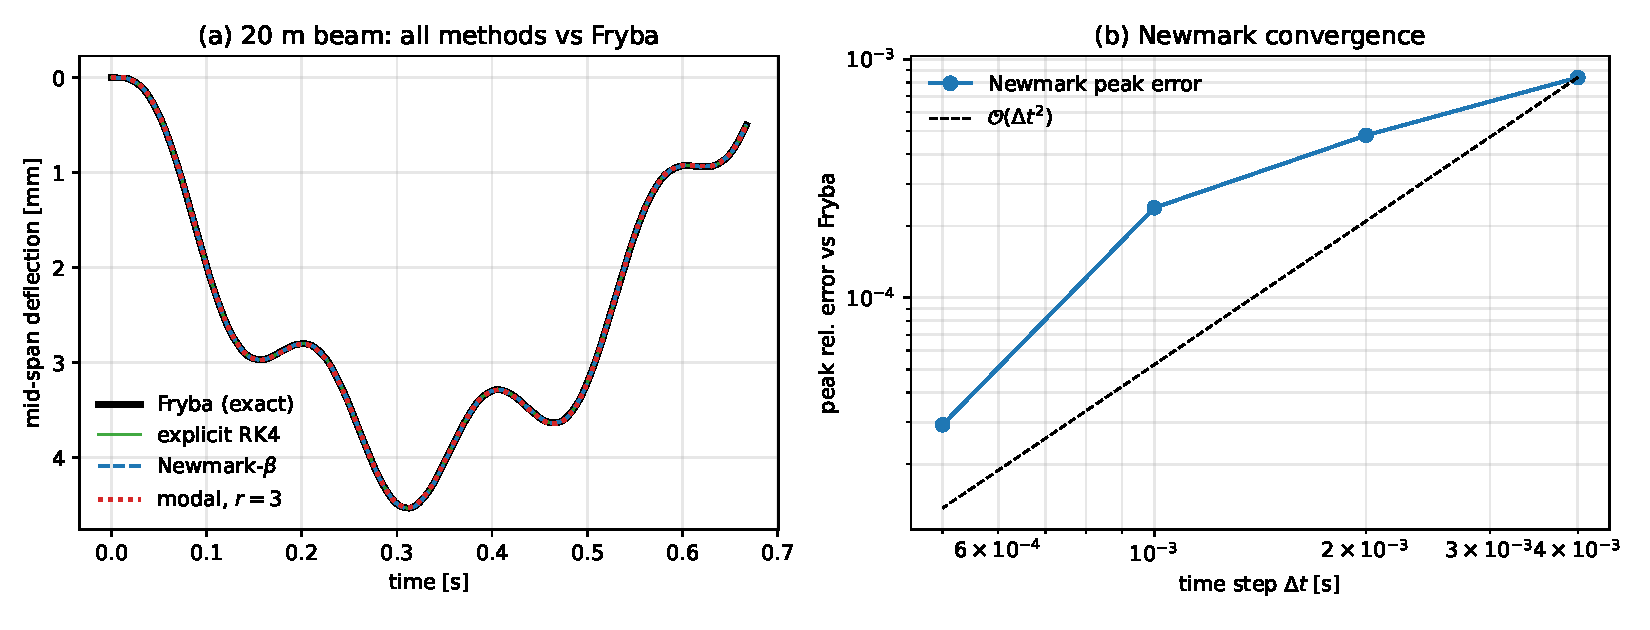
\includegraphics[width=\textwidth]{validation.pdf}
  \caption{(a) Mid-span deflection of the \SI{20}{m} beam at \(v=\SI{30}{m/s}\):
  explicit RK4, Newmark-\(\beta\) and the three-mode reduced model all sit on the
  Fr\'yba exact curve. (b) Newmark peak-deflection error against Fr\'yba versus
  step size, confirming the expected \(\mathcal O(\Delta t^2)\).}
  \label{fig:validation}
\end{figure}

\begin{figure}[t]
  \centering
  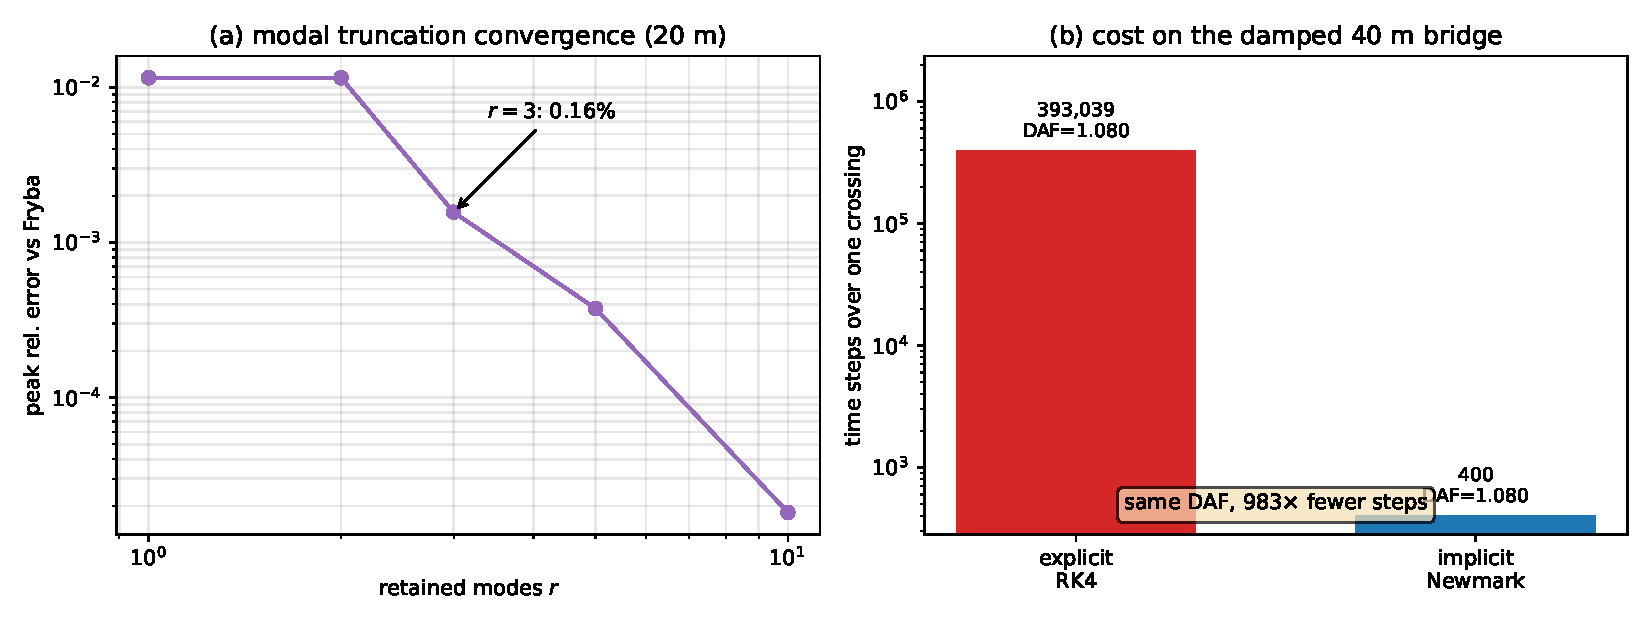
\includegraphics[width=\textwidth]{remedies.pdf}
  \caption{(a) Modal-truncation convergence on the \SI{20}{m} beam: three modes
  reach \(0.16\,\%\). (b) Cost on the damped \SI{40}{m} bridge: implicit Newmark
  reaches the same DAF as explicit RK4 with \(983\times\) fewer steps.}
  \label{fig:remedies}
\end{figure}

% ===========================================================================
\section{Limitations and scope}
% ===========================================================================
The model is deliberately the simplest one that exhibits the effect: a linear,
single-span Euler--Bernoulli beam under a constant moving force with classical
Rayleigh damping. The step restriction \eqref{eq:damped-cap} is a known property
of explicit integrators applied to stiffly damped systems; this note quantifies
it in the moving-load setting and checks the two standard remedies against the
Fr\'yba reference. Mass-proportional
damping (\(\alpha\mathbf M\)) does not cause the restriction; it is specific to
the \(\beta\mathbf K\) term. For nonlinear vehicle--bridge coupling or
multi-span continuous girders the same reasoning applies to the linearised
high-frequency content, but the constants in \eqref{eq:ratio} would be
re-derived. Both remedies are standard: Newmark-\(\beta\) is the textbook
structural integrator and modal truncation is elementary model order reduction;
either one avoids the step restriction.

% ===========================================================================
\section*{Reproducibility}
% ===========================================================================
The beam FE core, the three integrators and the Fr\'yba reference are numpy-only.
Every figure and number in this note is regenerated by
\texttt{python note/make\_note\_figures.py}, which writes
\texttt{note/data.json}. Source:
\href{https://github.com/bypire/vbi-bridge-sim}{\texttt{github.com/bypire/vbi-bridge-sim}}.

\section*{Acknowledgement of tools}
AI assistance (Anthropic Claude) was used while preparing the code, figures and
text of this note. Every reported number is produced by the accompanying
\texttt{numpy}-only script; the author has checked the results and is
responsible for their correctness.

\begin{thebibliography}{9}
\setlength{\itemsep}{1pt}
\bibitem{fryba} L.~Fr\'yba, \emph{Vibration of Solids and Structures under Moving
  Loads}, 3rd ed., Thomas Telford, 1999.
\bibitem{newmark} N.~M.~Newmark, ``A method of computation for structural
  dynamics,'' \emph{J.\ Eng.\ Mech.\ Div.\ ASCE}, 85(3):67--94, 1959.
\bibitem{bathe} K.-J.~Bathe, \emph{Finite Element Procedures}, 2nd ed., 2014.
\bibitem{chopra} A.~K.~Chopra, \emph{Dynamics of Structures}, 4th ed.,
  Prentice Hall, 2012.
\bibitem{yang} Y.-B.~Yang, J.-D.~Yau, Y.-S.~Wu, \emph{Vehicle--Bridge Interaction
  Dynamics}, World Scientific, 2004.
\end{thebibliography}

\end{document}
